\subsection{Database Script}
\begin{figure}[htp]
\centering
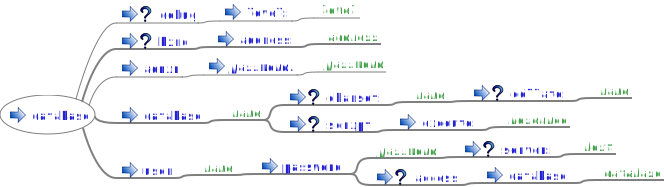
\includegraphics[width=0.9\textwidth]{database_service_script}
\label{fig:database_script_statements}
\caption{Database Script Statements}
\end{figure}


\TheStatement{database}
\TheStatement*[database]{database \{ debug bind admin database user \}}

Entry point in the database script.

\TheStatement[database:debug]{debug}
\TheStatement*[database!debug]{debug name, [level: \Arg{level}] [file: \Arg{file}]}

Sets the debug logging \Arg{level} and logging \Arg{file} for the database server. 
The \Arg{level} can be any positive number, zero is normally interpreted as no logging.

\begin{lstlisting}[style=Java]
database {
    debug "general", level: 1, file: "/var/log/mysql/mysql.log"
    debug "error", level: 1
    debug "slow-queries", level: 1
}
\end{lstlisting}

\TheStatement[database:bind]{bind}
\TheStatement*[database!bind]{bind local|all|\Arg{address} [, port: \Arg{port}]}

Sets the binding \Arg{address} and the binding \Arg{port}. Set to \qcode{local}
for the local host address \code{127.0.0.1} or to \qcode{all} to listen to all
hosts.

\begin{lstlisting}[style=Java]
database {
    bind "192.168.0.1", port: 3306
}
\end{lstlisting}

\TheStatement[database:admin]{admin}
\TheStatement*[database!admin]{admin password: \Arg{password}}

Sets the administrator \Arg{password} for the database server. If no password for
the administrator account was yet set this password is set. The administrator 
user is used to to create users, create databases and set permissions.

\begin{lstlisting}[style=Java]
database {
    admin password: "mysqladminpassword"
}
\end{lstlisting}

\TheStatement[database:db]{database}
\TheStatement*[database!database]{database \Arg{name} [, charset: \Arg{name}] [, collate: \Arg{name}] [, \{ script \}]}

Creates a new database with the specified database \Arg{name}, 
optionally set character set and collate. If the database was already on 
the server, the character set and collate should be updated to the specified 
character set and collate. The database server needs to support 
the specified character set and collate.

\begin{lstlisting}[style=Java]
database {
    database "postfixdb", charset: "latin1", collate: "latin1_swedish_ci"
}
\end{lstlisting}

\TheStatement[database:script]{script}
\TheStatement*[database!script]{script importing: \Arg{resource}}

Imports the script \Arg{resource}. The resource can be a file or URI. 
A string will be interpreted according to the format. If no scheme is used 
the string is assumed to be a local file.

\begin{lstlisting}[style=Java]
database {
    database "postfixdb", {
        script importing: "postfixtables.sql"
    }
}
\end{lstlisting}

\TheStatement[database:user]{user}
\TheStatement*[database!user]{user \Arg{name}, password: \Arg{password} [, server: \Arg{host}] [, \{ access \}]}

Creates a new user with the specified \Arg{name}, \Arg{password} and server \Arg{host}.
If the user already exists on the server, the password is updated for that user.
A user is identified by the user name and the server host.
The database that the user have read and write access to will be set. This will not create
the database on the server, to create a database use the \TheStatement*{database} statement.

\begin{lstlisting}[style=Java]
database {
    user "drupal6", password: "drupal6password", server: "srv2"
}
\end{lstlisting}

\TheStatement[database:access]{access}
\TheStatement*[database!access]{database: \Arg{database}}

Sets the access rights for the \Arg{database} for the user. The user is granted 
all permissions to the specified database.

\begin{lstlisting}[style=Java]
database {
    user "drupal6", {
        access database: "drupal6db"
    }
}
\end{lstlisting}

